\documentclass[11pt,a4paper]{article}

\usepackage[T1]{fontenc}
\usepackage[utf8]{inputenc}
\usepackage{amsmath,amsthm}
\usepackage{microtype}
\usepackage[margin=1in]{geometry}
\usepackage{array,booktabs,tabularx}
\usepackage[dvipsnames]{xcolor}
\usepackage{tikz}
\usetikzlibrary{positioning,arrows.meta,shapes.geometric,calc,fit,backgrounds,decorations.pathreplacing}
\usepackage{pgfplots}
\pgfplotsset{compat=1.18}
\usepackage{listings}
\usepackage[most]{tcolorbox}
\usepackage[font=small,labelfont=bf]{caption}
\usepackage{enumitem}
\usepackage[colorlinks,linkcolor=MidnightBlue,citecolor=MidnightBlue,urlcolor=MidnightBlue]{hyperref}
\usepackage[nameinlink]{cleveref}

% ---------------------------------------------------------------- notation
\newcommand{\cmb}[1]{\textsf{#1}}
\newcommand{\I}{\cmb{I}}
\newcommand{\K}{\cmb{K}}
\newcommand{\Sc}{\cmb{S}}
\newcommand{\B}{\cmb{B}}
\newcommand{\C}{\cmb{C}}
\newcommand{\Sp}{\cmb{S}'}
\newcommand{\Bs}{\cmb{B}^{*}}
\newcommand{\Cp}{\cmb{C}'}
\newcommand{\Y}{\cmb{Y}}
\newcommand{\IF}{\cmb{IF}}
\newcommand{\abs}[2]{[#1]\,#2}
\newcommand{\red}{\;\to\;}
\newcommand{\reds}{\;\to^{*}\;}

% graph = blue, spine = green, code = orange, heap = purple
\definecolor{tfill}{HTML}{DCE9F7}
\definecolor{sfill}{HTML}{DDF0DC}
\definecolor{cfill}{HTML}{FCE8D2}
\definecolor{hfill}{HTML}{F1DDEE}
\definecolor{tline}{HTML}{2F6DB5}
\definecolor{sline}{HTML}{3C8A3A}
\definecolor{cline}{HTML}{C7701C}
\definecolor{hline}{HTML}{9A3F8E}

\tikzset{
  >=Stealth,
  every picture/.append style={font=\small},
  ptr/.style={->, thick},
  half/.style={draw, minimum width=0.62cm, minimum height=0.55cm, inner sep=1pt, fill=white, font=\small\sffamily},
  newhalf/.style={half, fill=cfill},
  rooth/.style={half, fill=tfill},
  leaf/.style={inner sep=1.5pt, font=\small\sffamily},
  scell/.style={draw=sline, fill=sfill, minimum width=0.9cm, minimum height=0.5cm, font=\footnotesize, inner sep=1pt},
}
% \gcell[style]{name}{position}{fun}{arg}: an application cell of two halves,
% name-f and name-a
\newcommand{\gcell}[5][half]{%
  \node[#1, anchor=east] (#2-f) at (#3) {#4};
  \node[#1, anchor=west] (#2-a) at (#3) {#5};}

\theoremstyle{definition}
\newtheorem{definition}{Definition}
\newtheorem{exercise}{Exercise}
\theoremstyle{plain}
\newtheorem{theorem}{Theorem}

\newtcolorbox{aside}[1]{enhanced, breakable, colback=black!3, colframe=black!35,
  boxrule=0.5pt, arc=2pt, fonttitle=\bfseries\small, title={#1}, coltitle=black,
  colbacktitle=black!10, left=6pt, right=6pt}

\lstdefinelanguage{vm16}{morekeywords={LI,MOV,LW,SW,LB,SB,LWA,SWA,ADD,SUB,AND,OR,XOR,MUL,DIVU,
  NOT,NEG,SHL,SHR,SAR,ADDI,BEQ,BNE,BLT,BGE,BLTU,BGEU,BZ,BNZ,JMP,JR,PUSH,POP,GETDSP,SETDSP,
  GETRSP,CALL,CALLR,RET,SYS,HALT},
  sensitive=true, morecomment=[l]{;}}
\lstset{language=vm16, basicstyle=\ttfamily\small, keywordstyle=\bfseries,
  commentstyle=\color{black!55}, columns=fullflexible, keepspaces,
  frame=single, rulecolor=\color{black!30}, xleftmargin=6pt, xrightmargin=6pt,
  aboveskip=8pt, belowskip=8pt, tabsize=8}
\lstdefinestyle{plain}{language={}, keywordstyle={}}


\lstdefinelanguage{morc}{morekeywords={fn,if,then,else,true,false,nil},
  sensitive=true, morecomment=[l]{\#}}
\lstdefinestyle{morc}{language=morc, keywordstyle=\bfseries}

\newcommand{\tr}[1]{[\![#1]\!]}
\newcommand{\kw}[1]{\textbf{#1}}
\newcommand{\nt}[1]{\textit{#1}}

\title{MORC, the Mora Recursive Calculator\\[4pt]\large A small lazy language and its translation to combinator graphs}
\author{}
\date{\today}

\begin{document}
\maketitle

\begin{abstract}
\noindent
MORC is a small functional language with integers, functions and lists, in
the tradition of Turner's SASL and Miranda. It has named definitions, infix
operators with the usual precedences, \kw{if}--\kw{then}--\kw{else},
anonymous functions, and lazy evaluation. It has no run-time system of its own:
a MORC program is translated into a graph of Turner's combinators, which a
graph reducer of under two and a half kilobytes, written for the VM16
virtual machine,
rewrites into a result. This paper defines the language and follows a program
through every step of the translation: the tokens, the grammar and its
precedences, the reduction of the syntax to a core $\lambda$-calculus, bracket
abstraction, the linking of definitions into one cyclic graph, the text format
in which the graph is handed to the reducer, and the reduction itself. It ends
with measurements and with what the language still lacks.
\end{abstract}

\tableofcontents

% =====================================================================
\section{Introduction}\label{sec:intro}

A lazy functional language can be implemented in a surprisingly small amount
of code if one is willing to go through combinators. Turner's
SASL~\cite{turner79} and later Miranda~\cite{turner85} compiled a program into
a graph built from a handful of fixed functions, $\Sc$, $\K$, $\I$, $\B$,
$\C$ and a few more, and evaluated it by rewriting that graph in place. No
environments, closures or stack frames are needed; the graph is the whole
state of the computation.

MORC applies that idea to a machine with 64~kilobytes of memory. The
compiler runs on a host computer, in Python, and the reducer runs on
VM16, a 16-bit virtual machine designed to be implemented on 8-bit
processors such as the Z80. \Cref{fig:pipeline} shows the path of a program.
This is MORC's factorial:
\begin{lstlisting}[style=morc]
fn fac n = if n = 0 then 1 else n * fac (n - 1);
fn main = fac 7;
\end{lstlisting}
\begin{lstlisting}[style=plain]
$ ./run fac.morc
5040
[87 reductions, 0 collections]
\end{lstlisting}
The rest of the paper explains what happens between those two listings.
\Cref{sec:language} introduces the language through examples,
\cref{sec:lexical,sec:grammar} define its tokens and grammar, and
\cref{sec:meaning} its meaning. \Cref{sec:core,sec:abstraction,sec:linking}
give the translation: from MORC to a core $\lambda$-calculus, from there to
combinators, and from a set of definitions to one graph.
\Cref{sec:format,sec:reduction} show how the graph reaches the reducer and
how it is reduced, \cref{sec:measure,sec:lacks} measure the result and
discuss what is missing, and \cref{sec:future} plans the road to a compiler
written in MORC. A companion tutorial~\cite{graphtut} explains
combinator graph reduction itself in more depth.

\begin{figure}[t]
\centering
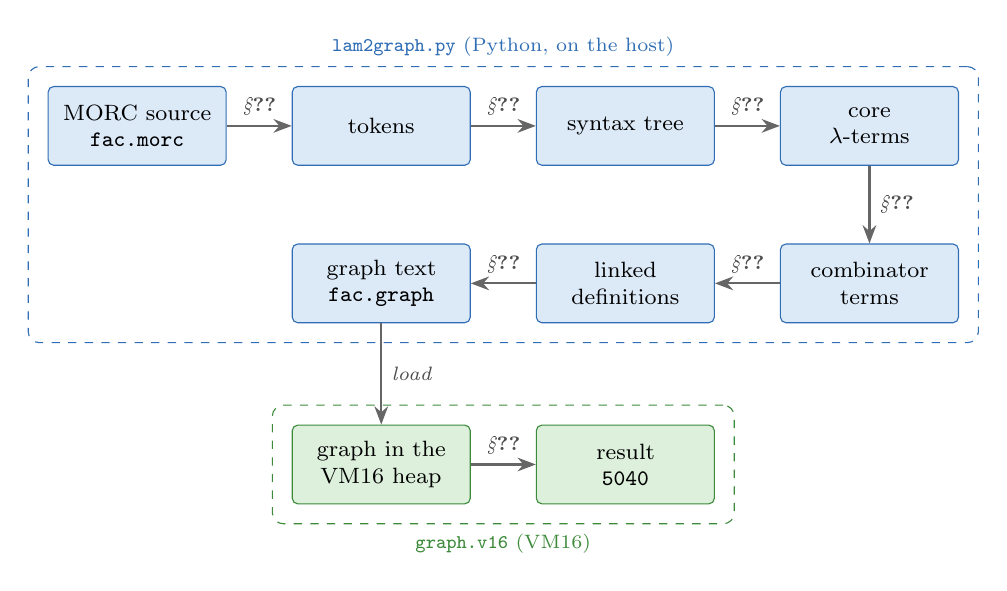
\begin{tikzpicture}[
  stage/.style={draw, rounded corners=2pt, align=center, font=\footnotesize,
                minimum height=1.0cm, inner sep=3pt, text width=2.05cm},
  host/.style={stage, fill=tfill, draw=tline},
  target/.style={stage, fill=sfill, draw=sline},
  flow/.style={->, thick, black!60},
  lab/.style={font=\scriptsize\itshape, black!70, align=center}]
\node[host] (src) at (0,0) {MORC source\\\texttt{fac.morc}};
\node[host] (tok) at (3.1,0) {tokens};
\node[host] (ast) at (6.2,0) {syntax tree};
\node[host] (core) at (9.3,0) {core\\$\lambda$-terms};
\node[host] (comb) at (9.3,-2.0) {combinator\\terms};
\node[host] (link) at (6.2,-2.0) {linked\\definitions};
\node[host] (txt) at (3.1,-2.0) {graph text\\\texttt{fac.graph}};
\node[target] (heap) at (3.1,-4.3) {graph in the\\VM16 heap};
\node[target] (res) at (6.2,-4.3) {result\\\texttt{5040}};
\draw[flow] (src) -- node[lab, above] {\S\ref{sec:lexical}} (tok);
\draw[flow] (tok) -- node[lab, above] {\S\ref{sec:grammar}} (ast);
\draw[flow] (ast) -- node[lab, above] {\S\ref{sec:core}} (core);
\draw[flow] (core) -- node[lab, right] {\S\ref{sec:abstraction}} (comb);
\draw[flow] (comb) -- node[lab, above] {\S\ref{sec:linking}} (link);
\draw[flow] (link) -- node[lab, above] {\S\ref{sec:format}} (txt);
\draw[flow] (txt) -- node[lab, right] {load} (heap);
\draw[flow] (heap) -- node[lab, above] {\S\ref{sec:reduction}} (res);
\begin{scope}[on background layer]
\node[draw=tline, dashed, rounded corners, fit=(src)(core)(comb)(txt), inner sep=7pt,
  label={[font=\scriptsize, tline]north:\texttt{lam2graph.py} (Python, on the host)}] {};
\node[draw=sline, dashed, rounded corners, fit=(heap)(res), inner sep=7pt,
  label={[font=\scriptsize, sline]south:\texttt{graph.v16} (VM16)}] {};
\end{scope}
\end{tikzpicture}
\caption{The path of a MORC program. Everything up to the graph text happens
on the host, in \texttt{lam2graph.py} and \texttt{morc.py}; the reducer on
VM16 only loads a graph and rewrites it. \texttt{run} does both steps.}
\label{fig:pipeline}
\end{figure}

\paragraph{Where MORC comes from.} The name stands for \emph{Mora Recursive
Calculator}. MORC began as a grammar sketched some years before this
implementation, with \kw{fn} definitions, \kw{if}--\kw{then}--\kw{else} and
infix operators. The version described here keeps that surface and settles
the details the sketch left open, chiefly the precedence of function
application, in the way most functional languages do. The same compiler
also reads a terser notation, the \texttt{.lam} files of the companion
tutorials, in which MORC's factorial is written
\verb|fac n = if n == 0 then 1 else n * fac (n-1); fac 7|. Both produce the
same syntax tree, and everything after the reader is shared.

% =====================================================================
\section{The language by example}\label{sec:language}

A MORC program is a series of definitions, each introduced by \kw{fn} and
ended by a semicolon. The value of the program is the value of \textit{main}.

\paragraph{Functions on numbers.} Numbers are integers, and functions are
defined by naming their parameters:
\begin{lstlisting}[style=morc]
fn fib n = if n < 2 then n else fib (n - 1) + fib (n - 2);
fn main = fib 20;
\end{lstlisting}
Function application is written by juxtaposition and binds tighter than any
operator, so the \kw{else} branch adds the results of two calls. A definition may
use itself, and definitions may use each other in any order.

\paragraph{Functions as values.} A function can be passed, returned and
written anonymously with a backslash and an arrow:
\begin{lstlisting}[style=morc]
fn twice f x = f (f x);
fn main = twice (\x -> x * 2) 3;          # 12
\end{lstlisting}
Every function takes its arguments one at a time, so \verb|twice (\x -> x * 2)|
is itself a function, waiting for its second argument. An operator in
brackets is a function of two arguments: \verb|(+) 3 4| is 7.

\paragraph{Lists.} \verb|h : t| is a list with head $h$ and tail $t$, and
\kw{nil} is the empty list. A list is taken apart by applying it to two
things: a function of the head and the tail, used if the list is not empty,
and a value to give if it is:
\begin{lstlisting}[style=morc]
fn length l = l (\h t -> 1 + length t) 0;
fn main = length (1 : 2 : 3 : nil);       # 3
\end{lstlisting}

\paragraph{Laziness.} An argument is evaluated only when its value is needed,
and then only once. Lists can therefore be infinite, as long as only a finite
part of them is used. This program finds the 100th prime by filtering the
infinite list of integers from 2:
\begin{lstlisting}[style=morc]
fn from n = n : from (n + 1);
fn filter p l = l (\h t -> if p h then h : filter p t else filter p t) nil;
fn sieve l = l (\h t -> h : sieve (filter (\x -> x % h != 0) t)) nil;
fn nth k l = l (\h t -> if k = 0 then h else nth (k - 1) t) 0;
fn primes = sieve (from 2);
fn main = nth 99 primes;                  # 541
\end{lstlisting}
\textit{primes} is a definition without parameters whose value is an infinite
list. It is computed only as far as \textit{nth} looks, and what has been
computed is kept and shared.

% =====================================================================
\section{Lexical structure}\label{sec:lexical}

A program is read as a sequence of tokens, separated by any amount of white
space. A \verb|#| starts a comment that runs to the end of the line. The
tokens are:

\begin{center}
\small
\begin{tabular}{@{}l l l@{}}
\toprule
token & form & examples\\
\midrule
name & a letter, then letters, digits and \verb|_| & \texttt{fac}, \texttt{x1}, \texttt{is\_even}\\
number & one or more digits & \texttt{0}, \texttt{16383}\\
keyword & \kw{fn if then else true false nil} & \\
operator & \verb|+ - * / % : = == != < <= > >=| & \\
punctuation & \verb|\ -> ( ) ;| & \\
\bottomrule
\end{tabular}
\end{center}

\noindent
Tokens are found by taking the longest match at each point, so \verb|<=| is
one token and \verb|n-1| is three. Keywords are names that cannot be used for
anything else. Numbers have 15 bits, the range the reducer stores
(\cref{sec:reduction}); a literal outside $-16384$ to $16383$ wraps around,
as arithmetic does. The tokens of the factorial program are
\begin{lstlisting}[style=plain]
fn fac n = if n = 0 then 1 else n * fac ( n - 1 ) ; fn main = fac 7 ;
\end{lstlisting}

% =====================================================================
\section{Grammar}\label{sec:grammar}

\Cref{fig:grammar} gives the grammar. Each level of \nt{expr} handles one
group of operators, from the loosest at the top to the tightest at the
bottom, which is the usual way of building precedence into a grammar for a
recursive-descent parser.

\begin{figure}[t]
\centering
\begin{tcolorbox}[enhanced, colback=black!2, colframe=black!35, boxrule=0.5pt,
  arc=2pt, width=0.95\textwidth, left=8pt, right=8pt]
\small
\renewcommand{\arraystretch}{1.15}
\begin{tabular}{@{}r@{\;\;}c@{\;\;}l@{}}
\nt{program} & ::= & \nt{definition} $\{$ \nt{definition} $\}$\\
\nt{definition} & ::= & \kw{fn} \textsc{name} $\{$ \textsc{name} $\}$ \texttt{=} \nt{expr} \texttt{;}\\[4pt]
\nt{expr} & ::= & \verb|\| \textsc{name} $\{$ \textsc{name} $\}$ \verb|->| \nt{expr}\\
 & $\mid$ & \kw{if} \nt{expr} \kw{then} \nt{expr} \kw{else} \nt{expr}\\
 & $\mid$ & \nt{compare}\\
\nt{compare} & ::= & \nt{cons} $[$ (\verb|=| $\mid$ \verb|==| $\mid$ \verb|!=| $\mid$ \verb|<| $\mid$ \verb|<=| $\mid$ \verb|>| $\mid$ \verb|>=|) \nt{cons} $]$\\
\nt{cons} & ::= & \nt{sum} $[$ \verb|:| \nt{cons} $]$\\
\nt{sum} & ::= & $[$ \verb|-| $]$ \nt{product} $\{$ (\verb|+| $\mid$ \verb|-|) \nt{product} $\}$\\
\nt{product} & ::= & \nt{app} $\{$ (\verb|*| $\mid$ \verb|/| $\mid$ \verb|%|) \nt{app} $\}$\\
\nt{app} & ::= & \nt{atom} $\{$ \nt{atom} $\}$\\
\nt{atom} & ::= & \textsc{name} $\mid$ \textsc{number} $\mid$ \kw{true} $\mid$ \kw{false} $\mid$ \kw{nil}\\
 & $\mid$ & \verb|(| \nt{expr} \verb|)| $\mid$ \verb|(| \nt{operator} \verb|)|\\
 & $\mid$ & \verb|\| \ldots{} $\mid$ \kw{if} \ldots \hfill (as in \nt{expr})\\
\end{tabular}

\medskip
\footnotesize
$\{\,x\,\}$ is zero or more $x$, and $[\,x\,]$ is an optional $x$. The
semicolon after the last definition may be left out.
\end{tcolorbox}
\caption{The grammar of MORC.}
\label{fig:grammar}
\end{figure}

\begin{table}[t]
\centering
\small
\begin{tabular}{@{}l l l l@{}}
\toprule
level & operators & grouping & example\\
\midrule
loosest & \verb|\x -> e|, \kw{if} & extend to the right & \verb|\x -> x + 1| is \verb|\x -> (x + 1)|\\
 & \verb|= == != < <= > >=| & none & \verb|a < b < c| is an error\\
 & \verb|:| & to the right & \verb|1 : 2 : nil| is \verb|1 : (2 : nil)|\\
 & \verb|+ -| & to the left & \verb|10 - 3 - 2| is 5\\
 & \verb|* / %| & to the left & \verb|1 + 2 * 3| is 7\\
tightest & application & to the left & \verb|f x y| is \verb|(f x) y|; \verb|f x + 1| is \verb|(f x) + 1|\\
\bottomrule
\end{tabular}
\caption{Precedence and grouping, loosest first. These are the conventions of
Haskell~\cite{haskell2010} and most other functional languages.}
\label{tab:precedence}
\end{table}

\Cref{tab:precedence} summarises the result. Several of the choices deserve a
comment.

\paragraph{Application binds tightest.} \verb|fac (n - 1)| is a call, and
\verb|n * fac (n - 1)| multiplies $n$ by it. The brackets are needed because
\verb|fac n - 1| would mean \verb|(fac n) - 1|. In \nt{app}, a sequence of
atoms is one application, grouped to the left, so \verb|f x y| applies
\verb|f x| to $y$.

\paragraph{Lambdas and conditionals extend to the right.} The body of
\verb|\x -> ...| and the \kw{else} branch of an \kw{if} are whole expressions,
so they reach as far right as they can: \verb|\x -> x + 1| is a function that
adds one, and \verb|if c then a else b + 1| adds one to $b$ only. Because a
lambda or an \kw{if} may also appear where an atom is expected, they need no
brackets as the last argument of a call or the right operand of an operator:
\verb|map \x -> x * 2| and \verb|1 + if c then 2 else 3| both parse as
expected. Nested conditionals chain without brackets:
\begin{lstlisting}[style=morc]
fn ack x y = if x == 0 then y + 1
             else if y == 0 then ack (x - 1) 1
             else ack (x - 1) (ack x (y - 1));
\end{lstlisting}

\paragraph{Comparisons do not chain.} \verb|a < b < c| is rejected rather than
read as \verb|(a < b) < c|, which would compare a truth value with $c$. MORC
accepts both \verb|=| and \verb|==| for equality. There is no ambiguity with
the \verb|=| of a definition, which can only follow \kw{fn} and the names of
the parameters.

\paragraph{Lists group to the right.} \verb|:| sits between the comparisons
and the arithmetic, so \verb|n + 1 : rest| puts $n+1$ in front of
\textit{rest}, and \verb|1 : 2 : nil| is a list of two elements.

\paragraph{Minus.} A \verb|-| at the start of a \nt{sum} is negation:
\verb|-x| is $0-x$, and \verb|-5| is the number $-5$. Elsewhere \verb|-| is
subtraction, so \verb|n-1| and \verb|n - 1| mean the same. To pass a negative
number as an argument it needs brackets, \verb|f (-1)|, since \verb|f -1| is
$f$ minus one.

\paragraph{Operators as functions.} An operator alone in brackets,
\verb|(+)|, \verb|(<=)| or \verb|(:)|, is the function of two arguments
that applies it.

\medskip
\noindent
The grammar can be read by a recursive-descent parser with one token of
lookahead, one procedure per level, and that is how \texttt{morc.py} reads
it. \Cref{fig:parse} shows the tree for the \kw{else} branch of the factorial.

\begin{figure}[t]
\centering
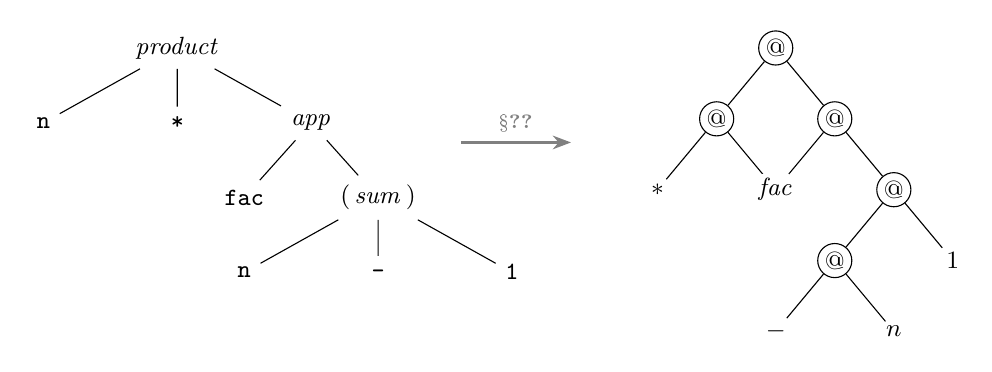
\begin{tikzpicture}[
  level distance=0.95cm,
  every node/.style={font=\small},
  nt/.style={font=\footnotesize\itshape, text=black!65},
  sibling distance=1.7cm]
\node {\nt{product}}
  child { node {\texttt{n}} }
  child { node {\texttt{*}} }
  child { node {\nt{app}}
    child { node {\texttt{fac}} }
    child { node {(\,\nt{sum}\,)}
      child { node {\texttt{n}} }
      child { node {\texttt{-}} }
      child { node {\texttt{1}} } } };
\begin{scope}[xshift=7.6cm, yshift=0cm, level distance=0.9cm, sibling distance=1.5cm,
  every node/.append style={fill=white, inner sep=1.5pt}]
\node[draw, circle, inner sep=1pt] {@}
  child { node[draw, circle, inner sep=1pt] {@}
    child { node {${*}$} }
    child { node {$n$} } }
  child { node[draw, circle, inner sep=1pt] {@}
    child { node {\textit{fac}} }
    child { node[draw, circle, inner sep=1pt] {@}
      child { node[draw, circle, inner sep=1pt] {@}
        child { node {${-}$} }
        child { node {$n$} } }
      child { node {$1$} } } };
\end{scope}
\draw[->, thick, black!50] (3.6,-1.2) -- node[above, font=\scriptsize] {\S\ref{sec:core}} (5.0,-1.2);
\end{tikzpicture}
\caption{\texttt{n * fac (n - 1)}: its parse tree (left), and the core term
it becomes (right), ${*}\;n\;(\mathit{fac}\;({-}\;n\;1))$, where every @ is an
application of its left child to its right.}
\label{fig:parse}
\end{figure}

% =====================================================================
\section{Meaning}\label{sec:meaning}

\paragraph{Values.} There are two kinds of value: integers and functions.
Integers have 15 bits, from $-16384$ to $16383$, and arithmetic wraps around.
\verb|/| and \verb|%| truncate towards zero, so \verb|-7 / 2| is $-3$ and
\verb|-7 % 2| is $-1$; dividing by zero stops the program.

\paragraph{Truth values} are numbers. The comparisons return 1 for true and
0 for false, \kw{true} and \kw{false} are 1 and 0, and \kw{if} takes its
\kw{then} branch for any number other than 0. A truth value can therefore be
used in arithmetic: \verb|count + (x > 0)|.

\paragraph{Lists} are functions. \verb|h : t| is the function that, given $c$
and $n$, returns $c\;h\;t$, and \kw{nil} is the function that returns $n$.
This is the \emph{Scott encoding} of lists. Taking a list apart is applying
it, as in \textit{length} above, and a list is printed as a function if it is
the result of the program.

\paragraph{Laziness.} An expression is evaluated only when its value is
needed: by an operator, which needs numbers; by \kw{if}, which needs its
condition; or by an application, which needs a function. Once evaluated, its
value replaces it, so it is never evaluated twice. In particular, the
branches of an \kw{if} need no special treatment: only the chosen one is ever
evaluated, because only it is needed.

\paragraph{Definitions} are evaluated at most once too. A definition with
parameters is a function; one without, such as \textit{primes}, is a value
that is computed the first time it is used and then kept for the rest of the
run.

\paragraph{Errors.} The compiler reports a syntax error with the token where
it occurred, an unbound name, a name defined twice, and a missing
\textit{main}. At run time the reducer stops with a message for division by
zero, an operator or \kw{if} given something other than a number, a number
applied as if it were a function, a value defined as itself
(\verb|fn x = x|), and running out of stack or memory.

% =====================================================================
\section{From MORC to the core}\label{sec:core}

The first step of the translation removes everything that is particular to
MORC. What remains is a small \emph{core} language, the untyped
$\lambda$-calculus with numbers and constants:
\[
  e \;::=\; x \;\mid\; n \;\mid\; c \;\mid\; e\;e \;\mid\; \lambda x.\,e
  \qquad c \in \{\,{+},\;{-},\;{*},\;{/},\;{\%},\;{=},\;{<},\;\IF\,\}.
\]
The constants are curried: ${+}\;a\;b$ adds $a$ and $b$, ${<}\;a\;b$ is 1 if
$a<b$ and 0 otherwise, and $\IF\;c\;t\;e$ is $t$ or $e$. This is the language
that the bracket abstraction of \cref{sec:abstraction} works on, and the
language of the \texttt{.lam} files.

\Cref{tab:core} gives the translation $\tr{\cdot}$. It works on the tree that
the parser builds and is applied to each definition in turn. Most of it is
direct: an infix operator becomes the corresponding constant applied to the
two operands, and \kw{if} becomes the constant $\IF$.

\begin{table}[t]
\centering
\small
\renewcommand{\arraystretch}{1.2}
\begin{tabular}{@{}l@{\quad}l@{}}
\toprule
MORC & core\\
\midrule
\kw{fn} $f\;x_1\ldots x_n$ \texttt{=} $e$ & $f = \lambda x_1.\ldots\lambda x_n.\,\tr{e}$\\
\verb|\|$x_1\ldots x_n$ \verb|->| $e$ & $\lambda x_1.\ldots\lambda x_n.\,\tr{e}$\\
$e_1\;e_2$ & $\tr{e_1}\;\tr{e_2}$\\
\kw{if} $c$ \kw{then} $a$ \kw{else} $b$ & $\IF\;\tr{c}\;\tr{a}\;\tr{b}$\\
$a$ \textit{op} $b$, for \textit{op} in \verb|+ - * / % = <| & $\textit{op}\;\tr{a}\;\tr{b}$\\
$a$ \verb|==| $b$ & ${=}\;\tr{a}\;\tr{b}$\\
$a$ \verb|>| $b$ & ${<}\;\tr{b}\;\tr{a}$\\
$a$ \verb|>=| $b$ & ${-}\;1\;({<}\;\tr{a}\;\tr{b})$\\
$a$ \verb|<=| $b$ & ${-}\;1\;({<}\;\tr{b}\;\tr{a})$\\
$a$ \verb|!=| $b$ & ${-}\;1\;({=}\;\tr{a}\;\tr{b})$\\
\verb|-|$a$ & ${-}\;0\;\tr{a}$, or the number $-n$ if $a$ is a number $n$\\
\kw{true}, \kw{false} & $1$, $0$\\
$a$ \verb|:| $b$ & $\mathit{cons}\;\tr{a}\;\tr{b}$\\
\kw{nil} & $\mathit{nil}$\\
\verb|(|\textit{op}\verb|)| & \textit{op}, or $\lambda a\,b.\,\tr{a\ \textit{op}\ b}$ if \textit{op} is not a constant\\
\midrule
built in & $\mathit{cons} = \lambda h\,t\,c\,n.\,c\;h\;t$ \qquad $\mathit{nil} = \lambda c\,n.\,n$\\
\bottomrule
\end{tabular}
\caption{The translation from MORC to the core language.}
\label{tab:core}
\end{table}

\paragraph{Four comparisons from two.} The reducer has only ${=}$ and ${<}$.
$a > b$ is $b < a$, with the operands swapped, and the other three negate a
comparison: $1 - (a < b)$ is $a \geq b$, since the comparison is 0 or 1. The
negation costs a subtraction at run time, which \cref{sec:measure} measures.
Swapping the operands of $>$ changes which operand is evaluated first. In a
language without side effects this cannot change a result, only which of
two errors is reported if both operands fail.

\paragraph{Lists from two definitions.} \textit{cons} and \textit{nil} are
ordinary definitions that the compiler adds to every program. Their names,
``\texttt{:}'' and ``\texttt{nil}'', cannot be written as MORC names, so they
cannot clash with the program's own, and like every other definition they
are only included in the output if the program uses them
(\cref{sec:linking}).

\paragraph{No new constructs.} Every MORC construct becomes a core term
built from things the reducer already has, so the reducer did not change
when MORC was added. This is also why MORC and the \texttt{.lam} notation can
share everything after the parser.

% =====================================================================
\section{Bracket abstraction}\label{sec:abstraction}

The core language still has variables and $\lambda$s, and the reducer has
neither. Bracket abstraction removes them. For a variable $x$ and a term $e$
without $\lambda$s, $\abs{x}{e}$ is a term without $x$ that, applied to $x$,
behaves like $e$:
\[
  \abs{x}{x} = \I \qquad
  \abs{x}{e} = \K\;e \ \ \text{($e$ any other variable or constant)} \qquad
  \abs{x}{(e_1\;e_2)} = \Sc\;(\abs{x}{e_1})\;(\abs{x}{e_2}),
\]
where $\I\,x = x$, $\K\,x\,y = x$ and $\Sc\,f\,g\,x = f\,x\,(g\,x)$. A term
$\lambda x.M$ is compiled by first compiling $M$, which removes the
$\lambda$s inside it, and then abstracting $x$.

These three rules alone produce large terms, so each $\Sc$ is simplified as it
is built, by Turner's rules~\cite{turner79}, tried in this order:
\[
\begin{array}{@{}l@{\qquad}l@{}}
\Sc\,(\K\,p)\,(\K\,q) = \K\,(p\,q) & \Sc\,(\B\,p\,q)\,(\K\,r) = \Cp\,p\,q\,r\\
\Sc\,(\K\,p)\,\I = p & \Sc\,p\,(\K\,q) = \C\,p\,q\\
\Sc\,(\K\,p)\,(\B\,q\,r) = \Bs\,p\,q\,r & \Sc\,(\B\,p\,q)\,r = \Sp\,p\,q\,r\\
\Sc\,(\K\,p)\,q = \B\,p\,q &
\end{array}
\]
The new combinators are defined by
\[
\begin{array}{@{}l@{\qquad}l@{}}
\B\,f\,g\,x = f\,(g\,x) & \Sp\,k\,f\,g\,x = k\,(f\,x)\,(g\,x)\\
\C\,f\,g\,x = f\,x\,g & \Bs\,k\,f\,g\,x = k\,(f\,(g\,x))\\
 & \Cp\,k\,f\,g\,x = k\,(f\,x)\,g
\end{array}
\]
and each one handles a common case directly: $\B$ when only the function
part of an application uses $x$, $\C$ when only the argument does, and the
primed versions for the same cases one level deeper. The companion
tutorial~\cite{graphtut} derives them and proves the rules correct.

Here is what some MORC fragments become, as \texttt{lam2graph.py -t} prints
them:
\begin{center}
\small
\begin{tabular}{@{}l l@{}}
\toprule
MORC & combinators\\
\midrule
\verb|\x y -> y x| & $\C\;\I$\\
\verb|fn twice f x = f (f x)| & $\Sc\;\B\;\I$\\
\verb|\x -> x * 2| & $\C\;{*}\;2$\\
\verb|fn f a b = a > b| & $\C\;{<}$\\
\verb|fn f a b = a <= b| & $\B\;(\B\;({-}\;1))\;(\C\;{<})$\\
\verb|fn f x = -x| & ${-}\;0$\\
\verb|fn len l = l (\h t -> 1 + len t) 0| & $\C\;(\C\;\I\;(\K\;(\B\;({+}\;1)\;\mathit{len})))\;0$\\
\textit{cons}, that is \verb|(:)| & $\Bs\;(\B\;(\B\;\K))\;\C\;(\C\;\I)$\\
\textit{nil} & $\K\;\I$\\
\midrule
\verb|fn fac n = if n = 0 then 1 else n * fac (n - 1)| & $\Sc\;(\Cp\;\IF\;(\C\;{=}\;0)\;1)\;(\Sc\;{*}\;(\B\;\mathit{fac}\;(\C\;{-}\;1)))$\\
\bottomrule
\end{tabular}
\end{center}
Applications group to the left, as in MORC. The factorial can be read from
the inside out: $\C\;{-}\;1$ is $\lambda n.\,n-1$, $\B\;\mathit{fac}\;(\C\;{-}\;1)$
is $\lambda n.\,\mathit{fac}\,(n-1)$, $\Sc\;{*}$ multiplies $n$ by that, and
$\Cp\;\IF\;(\C\;{=}\;0)\;1$ builds the conditional around it. Notice that
\textit{fac} and \textit{len} are still there, as names. They are not
variables of any $\lambda$, so abstraction treats them as constants. The next
section turns them into pointers.

% =====================================================================
\section{Linking definitions}\label{sec:linking}

A program is a set of definitions that refer to each other, while the reducer
needs a single graph. There are two ways to get from one to the other.

The first is to make the definitions into one big term. The program
\[
  \mathbf{fn}\ f_1 = e_1;\ \ldots;\ \mathbf{fn}\ f_n = e_n
\]
becomes $(\lambda f_1\ldots f_n.\,\mathit{main})\;e_1\ldots e_n$, with a
fixpoint combinator to let the $e_i$ refer to themselves. This is how the
early \texttt{.lam} programs were written, and it is expensive: bracket
abstraction must then pass every $f_i$ down through the whole program to each
place that uses it, and most of the compiled code is $\B$s and $\C$s doing
that routing.

The second, which SASL and Miranda used, is to keep the definitions apart.
Each $e_i$ is compiled on its own, leaving the names of definitions in it as
constants. Then each definition is given a cell in the heap, and every
occurrence of its name becomes a pointer to that cell. A recursive definition
becomes a cycle in the graph, and mutual recursion is simply a larger cycle,
so no fixpoint combinator is needed. \texttt{lam2graph.py} does this in four
steps.

\begin{enumerate}[itemsep=2pt]
\item \textbf{Check.} Every definition is compiled, and any name left free in
  it that is not a definition is reported as unbound, whether or not the
  definition is used.
\item \textbf{Number.} Starting from \textit{main}, definitions are numbered
  in the order in which they are first met: \textit{main} is 0, the first
  definition it uses is 1, and so on through the code of each numbered
  definition in turn. Definitions that are never reached get no number.
\item \textbf{Replace.} Each name in the compiled code is replaced by a
  reference to the number of its definition.
\item \textbf{Write.} The reachable definitions are written to the graph
  file, in the format of \cref{sec:format}.
\end{enumerate}

\noindent
The second step means that a program pays only for what it uses. A library
of definitions could be put in front of every program, and only the ones a
program reaches would be loaded. That is how \textit{cons} and \textit{nil}
are handled already.

\begin{figure}[t]
\centering
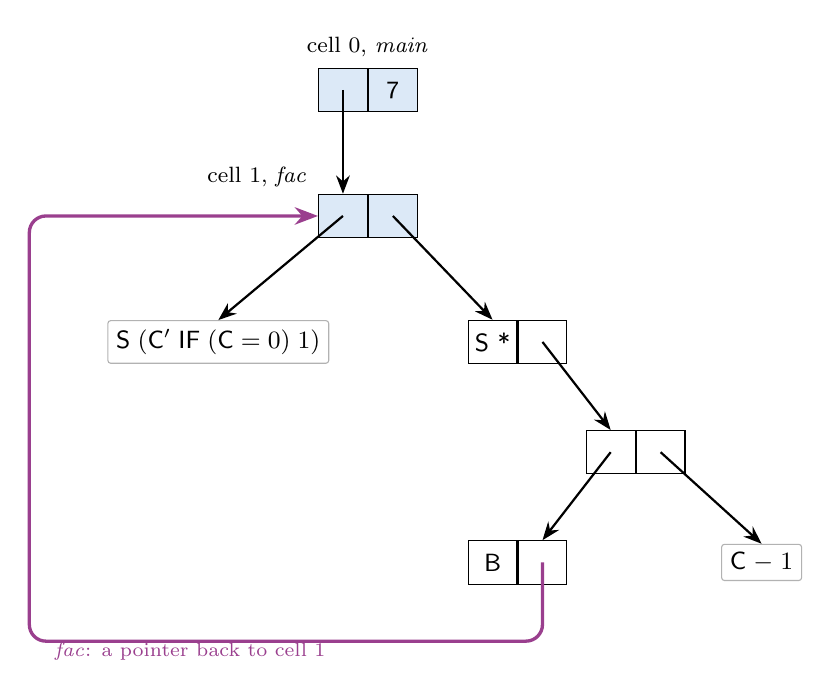
\begin{tikzpicture}[x=1cm, y=1cm]
\gcell[rooth]{m}{0,0}{}{\textsf{7}}
\node[font=\footnotesize, anchor=south] at (0,0.3) {cell 0, \textit{main}};
\gcell[rooth]{f}{0,-1.6}{}{}
\node[font=\footnotesize, anchor=south east] at (-0.65,-1.35) {cell 1, \textit{fac}};
\node[leaf, draw=black!30, rounded corners=1pt, inner sep=3pt] (left) at (-1.9,-3.2) {$\Sc\;(\Cp\;\IF\;(\C\;{=}\;0)\;1)$};
\gcell{a}{1.9,-3.2}{\textsf{S *}}{}
\gcell{b}{3.4,-4.6}{}{}
\gcell{c}{1.9,-6.0}{\textsf{B}}{}
\node[leaf, draw=black!30, rounded corners=1pt, inner sep=3pt] (cm) at (5.0,-6.0) {$\C\;{-}\;1$};
\draw[ptr] (m-f.center) -- (f-f.north);
\draw[ptr] (f-f.center) -- (left.north);
\draw[ptr] (f-a.center) -- (a-f.north);
\draw[ptr] (a-a.center) -- (b-f.north);
\draw[ptr] (b-f.center) -- (c-a.north);
\draw[ptr] (b-a.center) -- (cm.north);
\draw[ptr, hline, very thick, rounded corners=6pt] (c-a.center) -- ++(0,-1.0) -| (-4.3,-1.6) -- (f-f.west);
\node[font=\scriptsize, hline, align=left, anchor=north west] at (-4.1,-6.9) {\textit{fac}: a pointer back to cell 1};
\end{tikzpicture}
\caption{The factorial program after linking. Cell 1 holds the definition of
\textit{fac}, and the reference to \textit{fac} inside it, the argument of
$\B$, is a pointer back to the same cell: recursion is a cycle. Cell 0 holds
\textit{main}, \textit{fac}~7. Two subterms are drawn as boxes rather than as
cells.}
\label{fig:linked}
\end{figure}

\Cref{fig:linked} shows the factorial after linking. Two details matter for
the reducer.

\paragraph{Cells, not indirections.} The cell of a definition holds the
definition's top application itself, not a pointer to it. A reference to
\textit{fac} therefore leads straight to an $\Sc$ application, and the
reducer never has to step through an extra cell to find it. A definition
whose code is not an application, such as \verb|fn one = 1| or
\verb|fn main = f|, has no top cell to copy, so it is stored as $\I\;e$, which
costs one reduction the first time it is used.

\paragraph{Sharing comes for free.} Every use of a definition points at the
same cell, and the reducer overwrites a cell with its value when it reduces
it. A definition without parameters, like \textit{primes}, is therefore
evaluated once, the first time it is needed, and every later use sees the
part of it that has been computed so far. This is exactly the behaviour
described in \cref{sec:meaning}, and it costs nothing extra to implement.

% =====================================================================
\section{The graph file}\label{sec:format}

The compiler hands the linked graph to the reducer as text, in postfix: each
token pushes something on a stack, and the stack ends with the root of the
graph. The tokens are:

\begin{center}
\small
\begin{tabular}{@{}l l@{}}
\toprule
token & effect\\
\midrule
\verb|I K S B C S' B* C' Y IF + - * / % = <| & push the combinator\\
\verb|42|, \verb|-42| & push the number\\
\verb|@| & pop $a$ and $f$; push a new cell $(f, a)$, which is $f\;a$\\
\verb|%|$n$ & make $n$ cells for the definitions; must come first\\
\verb|$|$k$ & push the cell of definition $k$\\
\verb|=|$k$ & pop a cell; copy its two words into definition $k$'s cell\\
\verb|#| & a comment, to the end of the line\\
\bottomrule
\end{tabular}
\end{center}

\noindent
At the end of the file exactly one word must be left on the stack, the root
of the program. This is \texttt{fac.morc} compiled:
\begin{lstlisting}[style=plain]
%2
# main
$1 7 @ =0
# fac
S C' IF @ C = @ 0 @ @ 1 @ @ S * @ B $1 @ C - @ 1 @ @ @ @ =1
# the program
$0
\end{lstlisting}
The first line makes two cells. \verb|$1 7 @ =0| builds \textit{fac}~7 and
stores it in cell 0, \textit{main}. The next line builds the code of
\textit{fac} and stores it in cell 1; inside it, \verb|B $1 @| is
$\B\;\mathit{fac}$ with a pointer to cell 1, which makes the cycle of
\cref{fig:linked}. Note that \verb|$1| is used on the line of \textit{main}
before cell 1 has been filled. That is allowed, since a reference only needs
the address of the cell, and the cell exists from the first line.

\paragraph{The loader.} \texttt{graph.asm} reads this format with a loop
of about 160 VM16 instructions, including the input routines it shares with
the rest of the reducer. The heap is empty when loading starts, so the $n$
cells made by \verb|%|$n$ are the first $n$ cells of the heap, and cell $k$
is at a fixed address, $\mathit{HEAP} + 4k$. \verb|$|$k$ is a single
computation, and the loader needs no symbol table and no second pass. The
numbers are chosen by the compiler, so names never reach the target machine.

\paragraph{Why text.} A binary image of the heap would be smaller and faster
to load. Text has three advantages: it can be read and written by hand, as
in the tests of the loader; it does not depend on the reducer's memory
layout; and it can be produced by a very simple program, including, one day,
a compiler written in MORC itself (\cref{sec:future}).

% =====================================================================
\section{Reduction}\label{sec:reduction}

The reducer represents every value in one 16-bit word: a number $n$ as the
odd word $2n+1$, a combinator as a small even code, and a cell as its even
address in the heap. Cells are two words, the function and the argument of an
application, with no tag. The reducer finds the leftmost combinator by
following the function parts from the root, pushing each cell on a stack (the
\emph{spine}), and if the combinator has all its arguments, it rewrites the
root of that application with the right-hand side of the combinator's rule.
The details are in the companion tutorial~\cite{graphtut}; here is what
happens to MORC's factorial of 2, as \texttt{prototype.py -{}-trace} prints
it. Each line shows the graph after one reduction, and \verb|@| marks the
pointer back to the cell of \textit{fac}.

\begin{lstlisting}[style=plain, basicstyle=\ttfamily\footnotesize]
 0      S (C' IF (C = 0) 1) (S * (B @ (C - 1))) 2
 1  S   C' IF (C = 0) 1 2 (S * (B (S (C' IF (C = 0) 1) @) (C - 1)) 2)
 2  C'  IF (C = 0 2) 1 (S * (B (S (C' IF (C = 0) 1) @) (C - 1)) 2)
 3  C   IF (= 2 0) 1 (S * (B (S (C' IF (C = 0) 1) @) (C - 1)) 2)
 4  =   IF (I 0) 1 (S * (B (S (C' IF (C = 0) 1) @) (C - 1)) 2)
 5  IF  I (S * (B (S (C' IF (C = 0) 1) @) (C - 1)) 2)
 6  S   I (* 2 (B (S (C' IF (C = 0) 1) (S * @)) (C - 1) 2))
 7  B   I (* 2 (S (C' IF (C = 0) 1) (S * (B @ (C - 1))) (C - 1 2)))
 ...
25  IF  I (* 2 (I (* (I 1) (I 1))))
26  *   I (* 2 (I (I 1)))
27  *   I (I 2)
\end{lstlisting}

\noindent
Steps 1 to 5 are the test $n = 0$. $\Sc$ passes $n$ to both halves of the
definition, $\Cp$ and $\C$ route it into the comparison, the comparison
yields 0 (written $\I\,0$, an indirection to the value), and $\IF$ chooses the
\kw{else} branch. Steps 6 and 7 build $2 * \mathit{fac}\,(2-1)$; at step 7 the
$\B$ reaches the pointer to \textit{fac} and applies the definition's own
cell to the argument, which is the recursive call. The same pattern repeats
for $n=1$, and the multiplications finish the job. The argument $2-1$ is
built once, as the cell \verb|C - 1 2|, and shared by the comparison and the
recursive call: at step 12 it is reduced to 1, and both uses see the result.

% =====================================================================
\section{Measurements}\label{sec:measure}

\Cref{tab:measure} compares the MORC versions of three programs with the
\texttt{.lam} versions of the companion tutorial, which are written in the
terser notation but compute the same thing in the same way. The cells are the
application cells of the compiled code, not counting the cell of each
definition, and the VM16 instructions are counted by the C interpreter, split
into loading the graph (\emph{setup}) and everything after (\emph{run}).

\begin{table}[t]
\centering
\small
\begin{tabular}{@{}l l r r r r r@{}}
\toprule
 & & & & & \multicolumn{2}{c@{}}{VM16 instructions}\\
\cmidrule(l){6-7}
program & source & cells & reductions & GCs & setup & run\\
\midrule
$\mathit{fac}\ 7$ & \texttt{fac.morc} & 14 & 87 & 0 & 3,022 & 6,509\\
 & \texttt{fac.lam} & 14 & 87 & 0 & 2,725 & 6,509\\
\midrule
$\mathit{fib}\ 20$ & \texttt{fib.morc} & 19 & 240,795 & 45 & 3,717 & 16,796,640\\
 & \texttt{fib.lam} & 19 & 240,795 & 45 & 3,420 & 16,796,731\\
\midrule
100th prime & \texttt{primes.morc} & 72 & 177,761 & 49 & 12,680 & 13,146,080\\
 & \texttt{primes.lam} & 65 & 154,682 & 43 & 11,288 & 10,692,216\\
\bottomrule
\end{tabular}
\caption{MORC and \texttt{.lam} versions of the same programs.}
\label{tab:measure}
\end{table}

\paragraph{The same code.} For \textit{fac} and \textit{fib}, MORC produces
exactly the combinators of the \texttt{.lam} version and the same number of
reductions. The only difference is that \textit{main} is a definition of its
own, which costs one cell and a few hundred instructions of loading. The runs
of \textit{fib} differ by 91 instructions out of 16.8 million.

\paragraph{The cost of !=.} \texttt{primes.morc} tests divisibility with
\verb|x % h != 0|, which becomes
\[
  {-}\;1\;({=}\;({\%}\;x\;h)\;0),
\]
while
\texttt{primes.lam} uses the remainder directly as the condition. The extra
comparison and subtraction, and the combinators that route their arguments,
cost 15\,\% more reductions and 23\,\% more instructions. Writing
\verb|if x % h then ...| in MORC would give the same code as the
\texttt{.lam} version, since any number other than 0 counts as true; the
cleaner test is the one most programmers would write, and a compiler that
simplified ${-}\;1\;({=}\;e\;0)$ in a condition (\cref{sec:lacks}) could get
the best of both.

\paragraph{Absolute speed.} At about 70 VM16 instructions per reduction, and
about 290 Z80 clock cycles per VM16 instruction, a 4\,MHz Z80 performs some
200 reductions per second. Factorial of 7 takes about 0.7 seconds there, and
the 100th prime would take about 16 minutes.

% =====================================================================
\section{What MORC lacks}\label{sec:lacks}

MORC is deliberately small, and several additions would make it more
pleasant without changing the reducer.

\paragraph{Pattern matching on lists.} Taking a list apart by applying it is
correct but hard to read. A construct such as
\begin{lstlisting}[style=morc]
fn length l = case l of nil -> 0 | h : t -> 1 + length t;
\end{lstlisting}
would translate directly into the application \verb|l (\h t -> 1 + length t) 0|.

\paragraph{Local definitions.} \kw{let} \ldots{} \kw{in} or \kw{where} would
allow helper functions and shared intermediate values inside a definition.
A non-recursive \kw{let} $x = a$ \kw{in} $b$ is $(\lambda x.\,b)\;a$; a
recursive one needs either a fixpoint combinator or lambda
lifting~\cite{pj87}, which turns local functions into global definitions with
extra parameters.

\paragraph{Characters, strings and output.} At present a program can only
produce a number. Turner's languages printed a lazy list of characters as it
was computed, which allows a program to produce output as it runs, and to
read its input the same way, as a lazy list that is filled in as it is
consumed. This needs two new combinators in the reducer, one to print an
element of the result list and one to read the next character, and
character literals in the language.

\paragraph{Simplification.} The compiler does no optimisation beyond Turner's
rules. The conditional \verb|if true then a else b| becomes $\IF\;1\;a\;b$,
not $a$, and a negated comparison used as a condition is computed in full. A
few rules applied to the core term before abstraction would remove both.

\paragraph{Types.} MORC is untyped, so \verb|1 2| and \verb|(\x -> x) + 1|
are only caught at run time. Hindley--Milner type inference, as in Miranda
and Haskell, would catch them at compile time, at the cost of a much larger
compiler.

\paragraph{A compiler in MORC.} The compiler is about 650 lines of Python.
With character input and output, it could be written in MORC itself,
compiled once by the Python version, and then run on the reducer. Compiling
the compiler with itself and comparing the result with the Python version's
output would be a strong test of both, and it would make the system
self-contained on the target machine, memory permitting: the reducer's heap
holds 4,608 cells, and a compiler would need a large part of them.

% =====================================================================
\section{Future work}\label{sec:future}

The aim of the project is a language that is small, yet expressive enough to
compile itself, with a translation from MORC to the $\lambda$-calculus and
from there to combinators that stays as straightforward as possible.
Efficiency comes second. Measured against that aim, the following changes
are planned, in order of importance. Most of them make things simpler; the
few additions are ones a compiler cannot do without.

\paragraph{One language, one job each.} At present there are two surface
syntaxes that overlap: MORC, and the \texttt{.lam} notation of the reducer's
tutorial~\cite{graphtut}, which has gained infix operators and
\kw{if}--\kw{then}--\kw{else}. Its reader is now the most complicated code in
the project: it looks ahead for \kw{then} to choose between two forms of
\kw{if}, decides whether a \texttt{-} starts a negative number by looking at
the token before it, and gives an operator one meaning at the start of an
application and another after an operand. None of that is instructive. The
plan is for MORC to be the only language programs are written in, and for
\texttt{.lam} to be exactly the core $\lambda$-calculus of
\cref{sec:core}: prefix operators, \verb|\x.|, \verb|if c t e| and nothing
else. It then becomes the visible intermediate language between MORC and the
combinators. Every stage of the compiler should be printable on its own:
\begin{lstlisting}[style=plain]
lam2graph.py --tokens | --tree | --core | --combinators  prog.morc
\end{lstlisting}
The core can be printed in \texttt{.lam} syntax and read back, which gives
a clean test of the first half of the compiler.

\paragraph{A smaller MORC.} Every construct is code that will later be
written again in MORC, so the language should keep only what earns its place:
\begin{itemize}
\item equality is \texttt{==} only, so that \texttt{=} always means a
  definition;
\item there are no negative literals: \texttt{-5} is unary minus applied to
  5, so the rule for minus does not depend on context;
\item sections such as \texttt{(>)} go, and can be defined in a prelude;
\item \kw{true} and \kw{false} stay only if they are used.
\end{itemize}
The keyword \kw{fn}, the semicolons, \kw{if}--\kw{then}--\kw{else},
\verb|\x -> e| and the precedence levels stay. They make the parser easy to
write by hand, and they are what makes the language pleasant to use.

\paragraph{Data types and \kw{case}.} A compiler is mostly trees and pairs.
A declaration and a matching \kw{case},
\begin{lstlisting}[style=morc]
data Expr = App f a | Lam x body | Var name | Num n;
fn size e = case e of App f a -> size f + size a
                    | Lam x b -> 1 + size b
                    | Var x   -> 1
                    | Num n   -> 1;
\end{lstlisting}
translate mechanically into the Scott encoding that MORC already uses for
lists. Each constructor becomes a definition,
\verb|App f a = \app lam var num -> app f a|, and the \kw{case} becomes an
application of the scrutinee to one function per alternative,
\verb|e (\f a -> ...) (\x b -> ...) ...|. This is also the best single
example of the whole approach. Lists then stop being built in:
\verb!data List = Nil | Cons h t!, with \texttt{:} as an operator for
\texttt{Cons}, belongs in the prelude.

\paragraph{A prelude.} A file \texttt{prelude.morc}, put in front of every
program, would hold lists, pairs, \texttt{map}, \texttt{foldr}, string
equality and similar functions. Linking already leaves out definitions that
are not reachable (\cref{sec:linking}), so the prelude costs nothing in
programs that do not use it.

\paragraph{Local definitions.} \kw{let} $x = a$ \kw{in} $b$ is just
$(\lambda x.\,b)\;a$. Recursive local functions can simply be disallowed and
written as global definitions instead, which keeps the translation trivial.

\paragraph{Characters, strings, input and output.} A character literal
\texttt{'a'} is a number, and a string \texttt{"fn"} is a list of numbers.
The lexer, the keyword tests and all of the compiler's output need them.
Following Turner, a program receives its input as a lazy list of characters,
and a result that is a list is printed character by character as it is
computed. This needs two or three new rules in \texttt{graph.asm}, the only
change to the reducer in the whole plan, and it fits lazy evaluation without
side effects.

\paragraph{The Python compiler as a blueprint.} At present
\texttt{prototype.py} combines the reader, the compiler, the linker, the
writer and a model of the reducer, using Python classes and mutable
dictionaries. It should be split into the stages of this paper and written in
the style the MORC version will have: pure functions, recursion over trees,
lists and pairs instead of dictionaries, and no updates in place. Porting it
then becomes almost line by line, and it remains the reference for the
bootstrap test below. The model of the reducer stays separate, since it
describes the machine, not the compiler.

\paragraph{Turner's rules as a separate pass.} Plain \Sc, \K{} and \I{} are
the part to teach, and they are easy to port. The rules for \B, \C, $\Sp$,
$\Bs$ and $\Cp$ (\cref{sec:abstraction}) belong in a separate peephole pass
over the result. That pass is short and can be explained on its own, and it
stays worth having, because memory, not speed, will be the limit.

\paragraph{Will it fit?} The reducer has 4,608 cells in each semispace. A
compiler written in MORC, plus a prelude, plus the program being compiled,
may well need more. Lazy evaluation also makes deep recursion over long lists,
such as a few thousand characters of source text, run out of stack. Before
the whole compiler is ported, a small part of it, such as the lexer, should be
written in MORC and run under \texttt{prototype.py} to measure the cells and
the nesting depth it needs. If it does not fit, the options are a larger heap
on the C implementation of VM16, which is enough for bootstrapping; a
mark-compact collector, which doubles the usable heap; and a strictness
primitive, \texttt{seq}, for accumulating parameters.

\paragraph{The bootstrap.} Once the compiler is written in MORC, the Python
compiler compiles it once, and the result runs on the reducer. Its output on
the test programs must equal the Python compiler's, and compiling the
compiler with itself must reproduce the same graph: a fixpoint. From then on
the system is self-contained on the target machine.

\paragraph{Order of work.}
\begin{enumerate}
\item \texttt{.lam} back to the plain core, and printable compiler stages.
\item The smaller MORC.
\item Data types, \kw{case}, the prelude and \kw{let}.
\item Characters, strings, and the input and output rules in the reducer.
\item The Python compiler restructured into purely functional stages.
\item The lexer in MORC, measured; then the rest of the compiler and the
  bootstrap test.
\end{enumerate}

% =====================================================================
\section{Summary}

MORC is a lazy functional language with a conventional surface, named
definitions, infix operators and \kw{if}--\kw{then}--\kw{else}, and almost
no machinery behind it. Its grammar is a standard precedence grammar with
application binding tightest. Its translation removes the surface syntax in
one table, removes variables by bracket abstraction with Turner's
combinators, and links definitions by pointers so that recursion becomes a
cycle in the graph. The result is handed to a graph reducer of 2.4 kilobytes
as postfix text. Each step is short, and only one of them, linking, needed
anything new on the target machine: three tokens in the reducer's loader.

% =====================================================================
\appendix
\section{Reference card}\label{sec:card}

\begin{center}
\small
\renewcommand{\arraystretch}{1.12}
\begin{tabular}{@{}p{0.46\textwidth}@{\quad}p{0.47\textwidth}@{}}
\toprule
\multicolumn{2}{@{}l}{\textbf{Programs}}\\
\verb|fn f x y = e;| & a definition; the program's value is \textit{main}\\
\verb|# ...| & a comment\\
\midrule
\multicolumn{2}{@{}l}{\textbf{Expressions}, loosest first}\\
\verb|\x y -> e| & a function; the body extends to the right\\
\verb|if c then a else b| & 0 is false, any other number true\\
\verb|a == b|, \verb|=|, \verb|!=|, \verb|<|, \verb|<=|, \verb|>|, \verb|>=| & comparisons, 1 or 0; they do not chain\\
\verb|h : t| & a list, grouped to the right\\
\verb|a + b|, \verb|a - b| & grouped to the left; \verb|-a| is negation\\
\verb|a * b|, \verb|a / b|, \verb|a % b| & \verb|/| and \verb|%| truncate towards zero\\
\verb|f x y| & application, \verb|(f x) y|; binds tightest\\
\verb|(e)|, \verb|(+)|, \verb|(:)| & brackets; an operator as a function\\
\verb|42|, \kw{true}, \kw{false}, \kw{nil} & 15-bit numbers; 1; 0; the empty list\\
\midrule
\multicolumn{2}{@{}l}{\textbf{Lists}}\\
\verb|l (\h t -> a) b| & $a$ with head $h$ and tail $t$ if $l$ is not empty, else $b$\\
\midrule
\multicolumn{2}{@{}l}{\textbf{Commands}}\\
\verb|./run prog.morc| & compile and run\\
\verb|python3 lam2graph.py -t prog.morc| & show the compiled combinators\\
\verb|python3 lam2graph.py prog.morc| & write \texttt{prog.graph}\\
\verb|python3 prototype.py --trace prog.morc| & the graph after every reduction\\
\bottomrule
\end{tabular}
\end{center}

% =====================================================================
\begin{thebibliography}{99}
\small

\bibitem{graphtut}
Combinator graph reduction: a tutorial introduction.
\newblock \texttt{graph/graph-tutorial.pdf} in this repository.

\bibitem{haskell2010}
S.~Marlow, editor.
\newblock \emph{Haskell 2010 Language Report}, 2010.

\bibitem{pj87}
S.~L. Peyton~Jones.
\newblock \emph{The Implementation of Functional Programming Languages}.
\newblock Prentice Hall, 1987.

\bibitem{turner79}
D.~A. Turner.
\newblock A new implementation technique for applicative languages.
\newblock \emph{Software---Practice and Experience}, 9(1):31--49, 1979.

\bibitem{turner85}
D.~A. Turner.
\newblock Miranda: a non-strict functional language with polymorphic types.
\newblock In \emph{Functional Programming Languages and Computer
  Architecture}, LNCS 201, pages 1--16. Springer, 1985.

\end{thebibliography}

\end{document}
